%! TEX program = xelatex
\documentclass{beamer}
\usepackage{graphicx}
\usetheme{metropolis}
\usepackage{listings}
\usepackage[scaled=0.85]{FiraMono}
\lstset{basicstyle=\ttfamily, keywordstyle=\bfseries}

\title{Trabajo Académico final}
\date{\today}
\author{Roberto Alvarado}
\institute{UTPL}
\begin{document}
  \maketitle
  \section{Dataset y presentación de datos}
  \begin{frame}[fragile]{Creación de base de datos}
      SQLITE, es una herramienta de manejo de bases de datos sql
\begin{lstlisting}
sqlite3 cancer.db
sqlite3> .mode csv
sqlite3> .import global.csv
sqlite3> .exit
\end{lstlisting}
    \end{frame}
    \begin{frame}[fragile]{Limpieza de datos}
        \scriptsize
    \begin{lstlisting}[language=Python]
//Eliminar columnas que no sirven
database_csv.loc[:,database_csv.columns != "Patient_ID"]
database_clean.loc[:,database_clean.columns != "Country_Region"]

//Conseguir el atributo objectivo
database_clean.loc[:,database_clean.columns == "Target_Severity_Score"]
    \end{lstlisting}
    \end{frame}
    \begin{frame}[fragile]{Analizar data}
        \scriptsize
    \begin{itemize}
        \item Explorar data
            \begin{lstlisting}[language=Python]
https://github.com/Kanaries/pygwalker
            \end{lstlisting}
        \item Hacerse preguntas
        \item Hacer diagramas para responder estas preguntas con diagramas
    \end{itemize}
    \end{frame}
  \begin{frame}{Global Cancer dataset 2019-2025}
      \center
      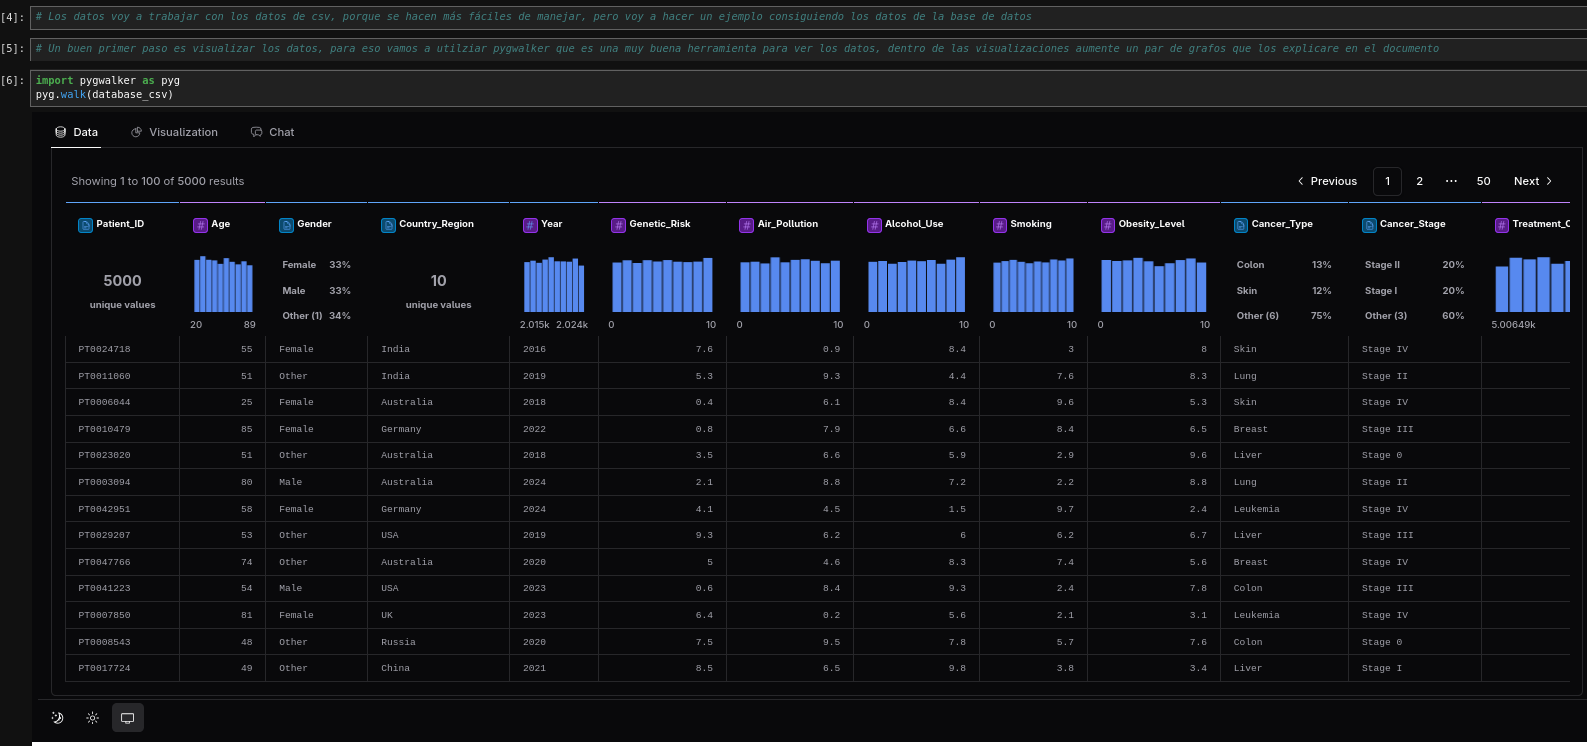
\includegraphics[width=\textwidth]{../figures/img0.png}
      Attributes ['Patient\_ID','Age', 'Gender', 'Year', 'Genetic\_Risk', 'Air\_Pollution', 'Alcohol\_Use',
      'Smoking', 'Obesity\_Level', 'Cancer\_Type', 'Cancer\_Stage',
      'Treatment\_Cost\_USD', 'Survival\_Years','Target\_Severity\_Rate']
  \end{frame}
    \begin{frame}[fragile]{¿Comó es la distribución de genéros de esta base datos?}
        \center
    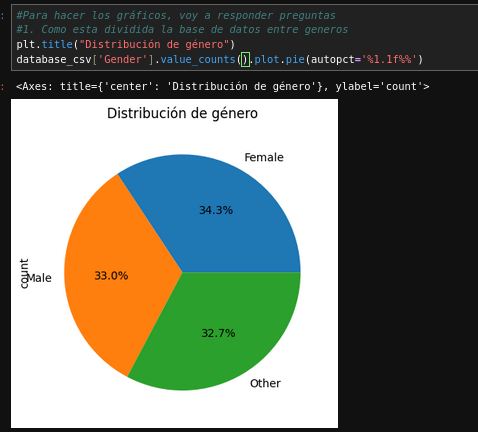
\includegraphics[width=0.8\textwidth]{../figures/img1.png}
    \end{frame}
    \begin{frame}[fragile]{¿Comó es la distribución de los tipos de cancer de esta base datos?}
        \center
    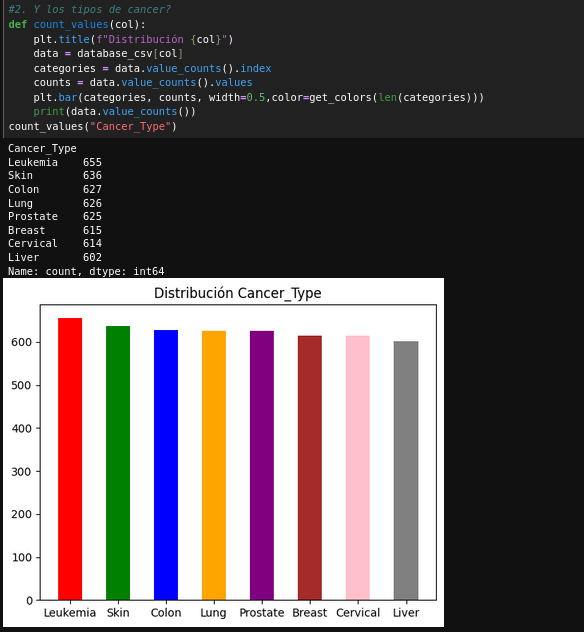
\includegraphics[width=0.6\textwidth]{../figures/img2.png}
    \end{frame}
    \begin{frame}[fragile]{¿Comó es la distribución de los resultados?}
    \center
    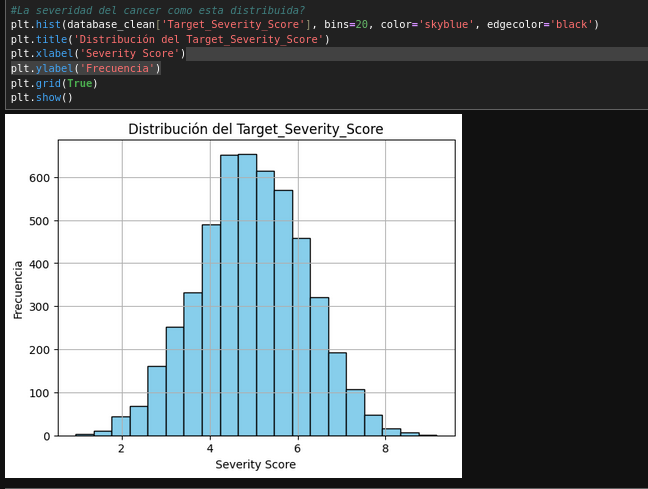
\includegraphics[width=0.7\textwidth]{../figures/img3.png}
    \end{frame}
    \begin{frame}[fragile]{¿Existen tipos de cancer en general más severo el uno de otro?}

    \scriptsize
    \begin{lstlisting}[language=Python]
cancer_types = database_clean['Cancer_Type'].unique()
cols = 4
rows = 2
fig, axes = plt.subplots(rows, cols, figsize=(20, 10))
for i, cancer in enumerate(cancer_types):
    ax = axes[i // cols, i % cols]
    sns.boxplot(data=database_clean[database_clean['Cancer_Type'] == cancer],
                y='Target_Severity_Score', ax=ax)
    ax.set_title(f'{cancer}')
    ax.set_ylabel("Severity Score")
plt.tight_layout()
plt.show()
    \end{lstlisting}
    \end{frame}
    \begin{frame}[fragile]{¿Existen tipos de cancer en general más severo el uno de otro?}
    \center
    \hspace*{-1cm}
    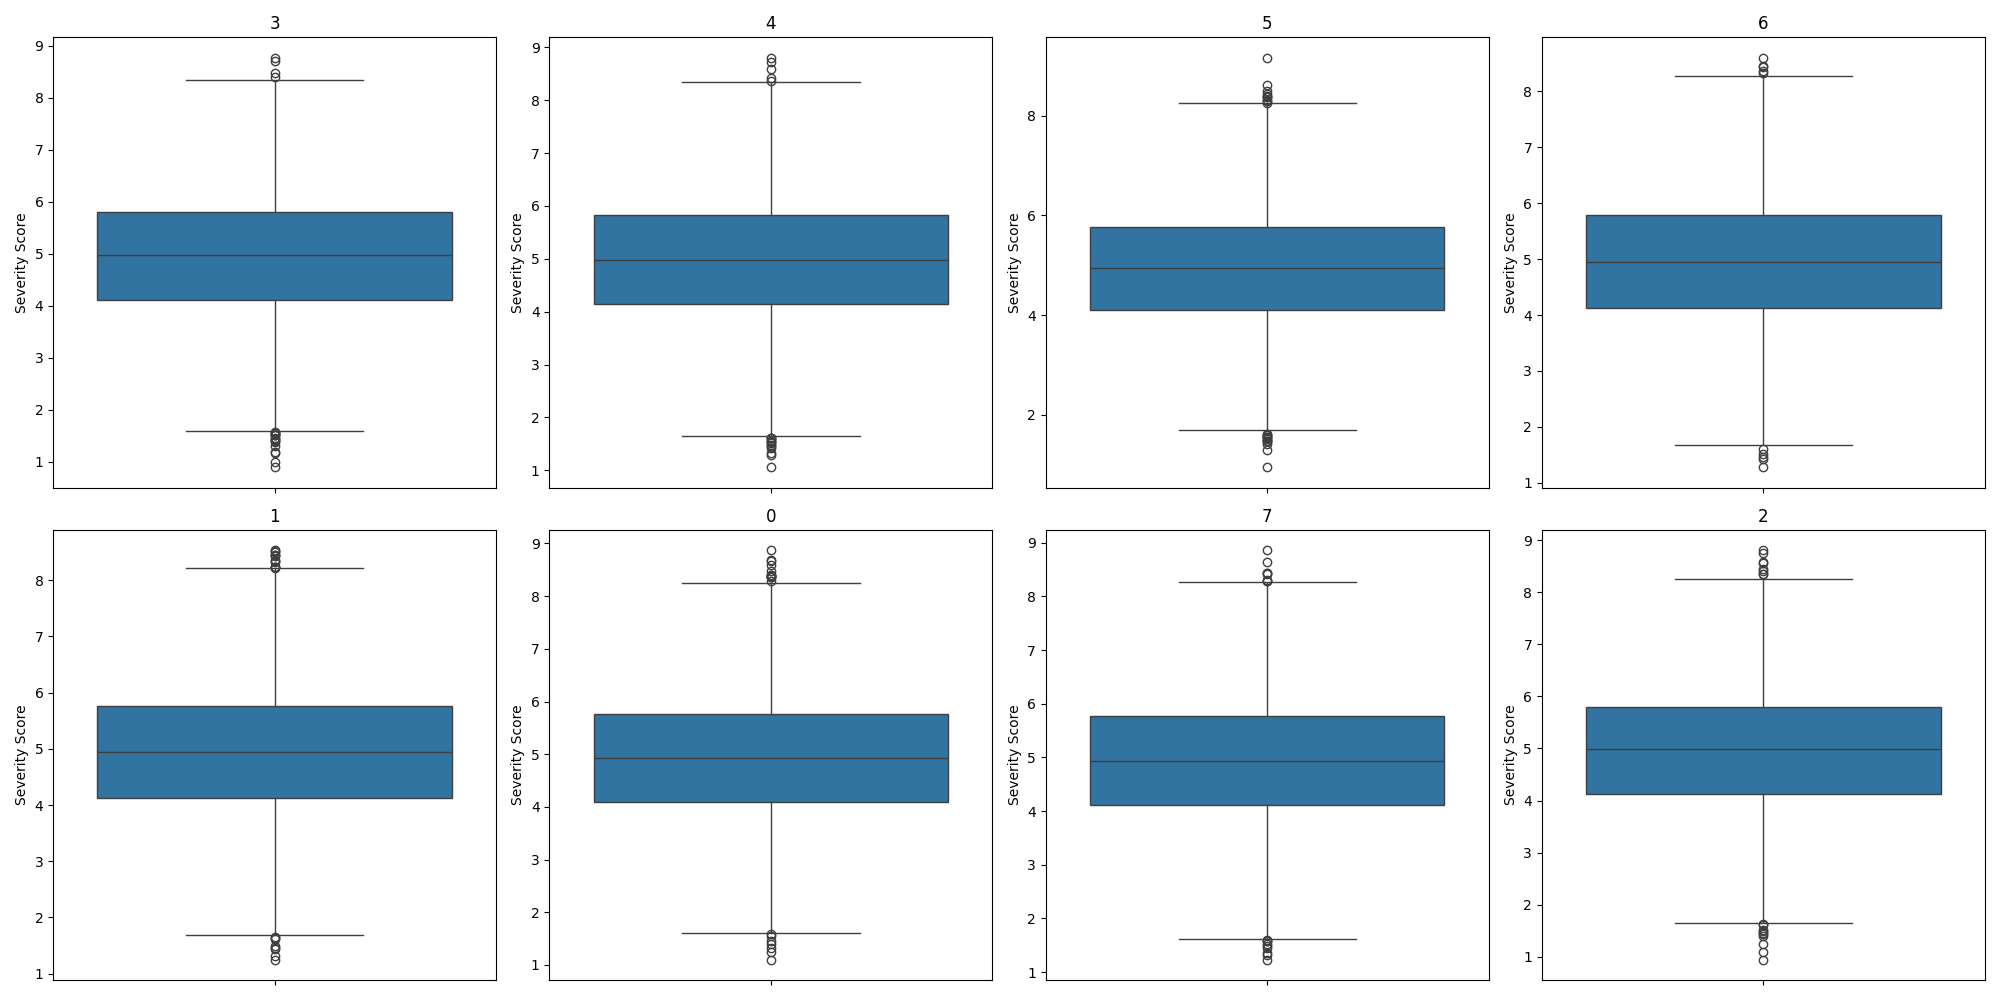
\includegraphics[width=1.16\textwidth,keepaspectratio]{../figures/img4.png}
    \end{frame}

    \begin{frame}[fragile]{ La severidad según la edad como se presenta }
        \tiny
    \begin{lstlisting}[language=Python]
cols = 4
rows = 2 fig, axes = plt.subplots(rows, cols, figsize=(16, 4 * rows))
fig.suptitle("Costos según tipo de cancer ")
for i, cancer in enumerate(cancer_types):
    ax = axes[i // cols, i % cols]
    subset = database_clean[database_clean['Cancer_Type'] == cancer]
    ax.hist(subset['Treatment_Cost_USD'], bins=10, color='steelblue', edgecolor='black')
    ax.set_title(f"{cancer} - Treatment Cost")
    ax.set_xlabel('USD')
    ax.set_ylabel('Count')

plt.tight_layout()
plt.savefig("./figures/img6.png")
plt.show()
    \end{lstlisting}
    \end{frame}
    \begin{frame}[fragile]{ La severidad según la edad como se presenta }
    \center
    \hspace*{-1cm}
    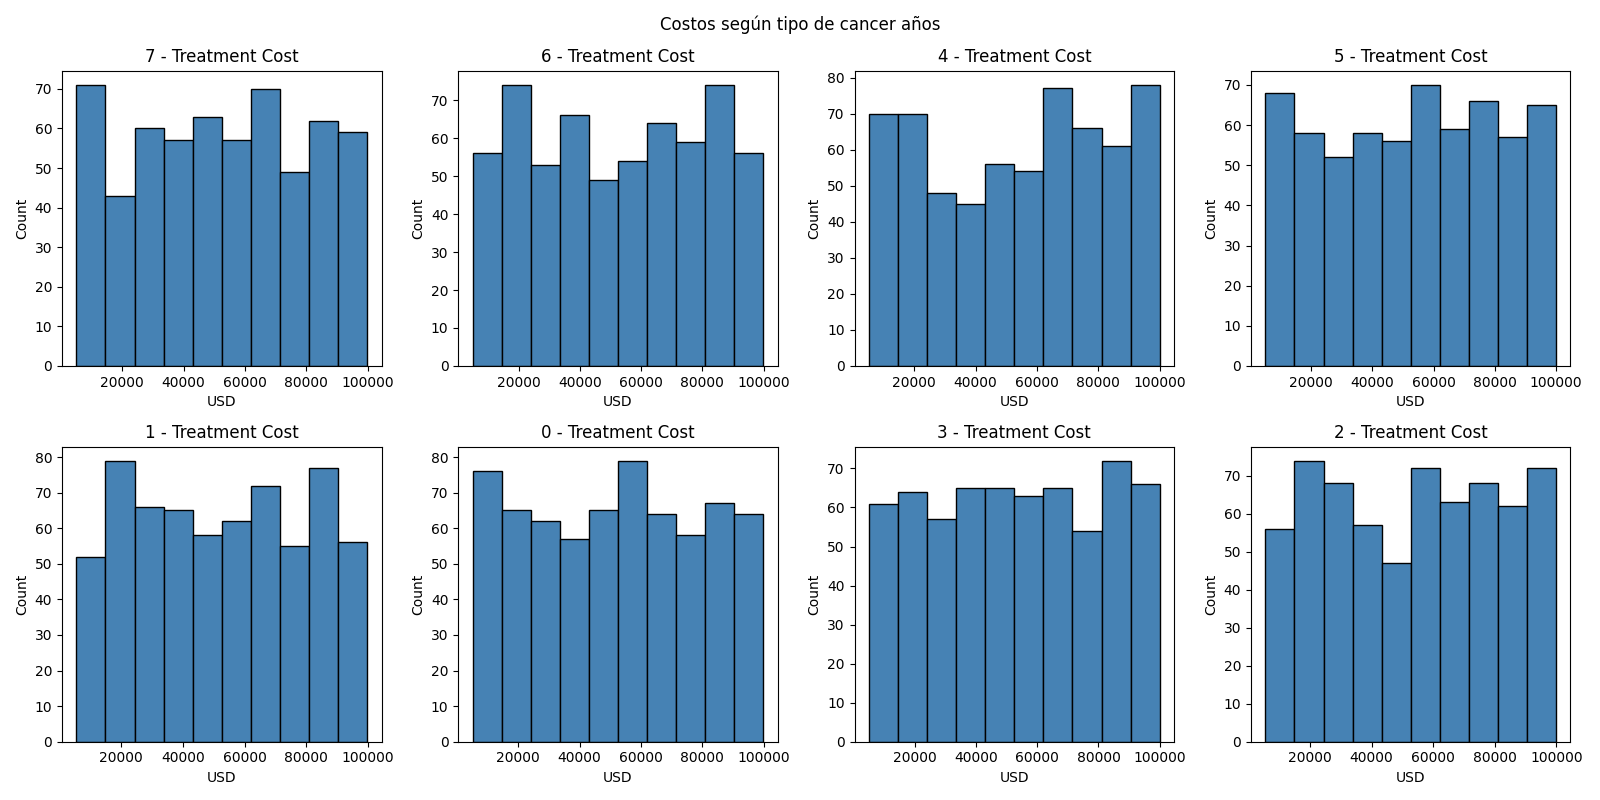
\includegraphics[width=1.16\textwidth,keepaspectratio]{../figures/img6.png}
    \end{frame}

    \begin{frame}[fragile]{¿Cuál es la relación entre obesidad y la severidad?}
    \center
    \hspace*{-1cm}
    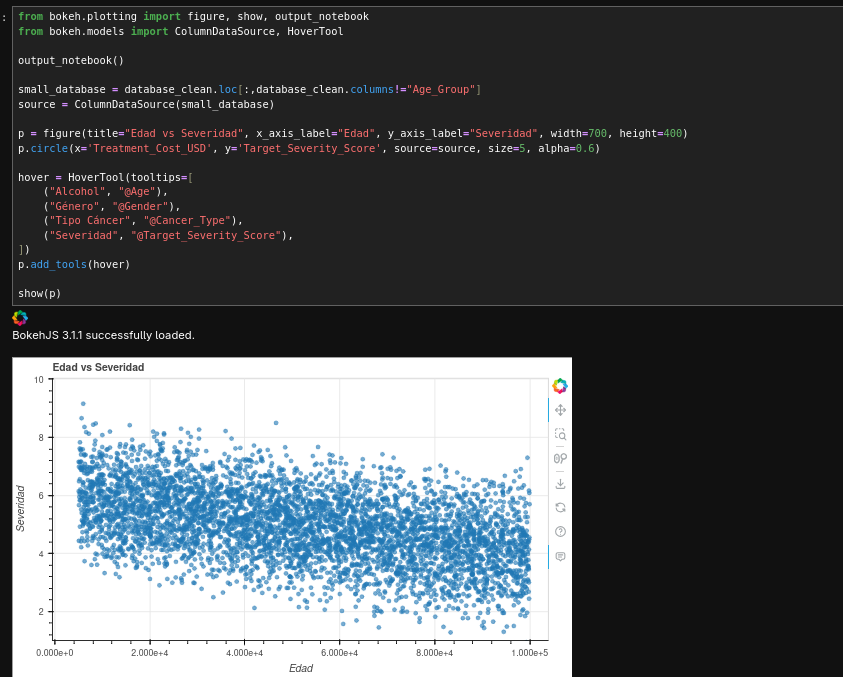
\includegraphics[width=0.8\textwidth,keepaspectratio]{../figures/img7.png}
    \end{frame}
    \begin{frame}[fragile]{¿Cuál es la relación entre el alcoholismo y la severidad?}
    \center
    \hspace*{-1cm}
    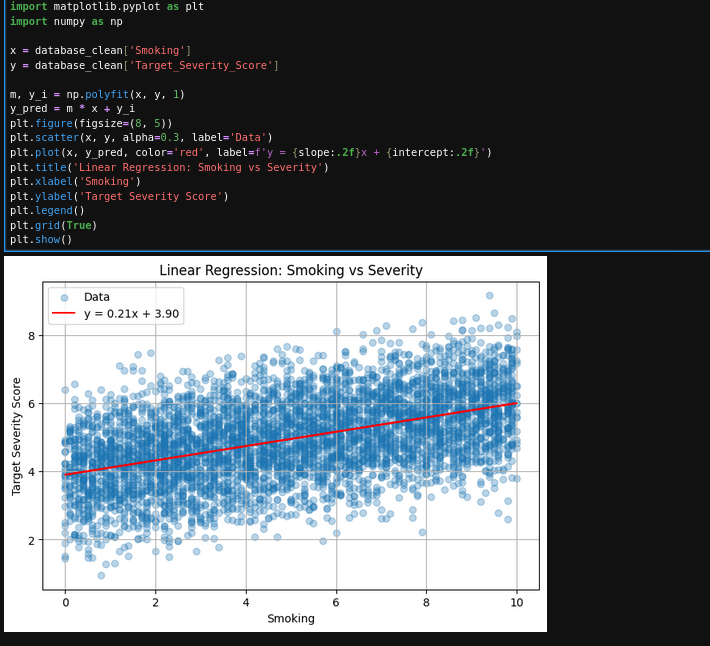
\includegraphics[width=0.8\textwidth,keepaspectratio]{../figures/img9.png}
    \end{frame}
\end{document}
